\section{Database}

\subsection{database}

	\begin{frame}{What?}
		\begin{block}{Metadata of task}<1->{}
		\begin{itemize}
		\item<1->{} {Identifier(ID)}
		\item<2->{} {Timestamp of an event}
		\item<3->{} {Event itself}
		\item<4->{} {Mode}
		\item<5->{} {Parent}
		\item<6->{} {Rank}
		
		%\item Intercommunication timestamp

		\item<7->{} {Number of parameters}
		\item<8->{} {Parameters themselves}
		\end{itemize}
		\end{block}
	\end{frame}
	
	\begin{frame}{How?}
		\begin{block}{Structure}<1->{}
		\begin{itemize}
		\item<1->{} {Stored data in 2 seperated files}
		\item<2->{} {Bookkeeping: listed data of previous slide}
		\item<3->{} {Statistics: parameters and runtime of a task}
		\item<5->{} {\textbf{Additional: }Files are accessable for visualizer}
		\end{itemize}
		\end{block}
	\end{frame}
\subsubsection{handling}
	\begin{frame}{DatabaseHandler}
	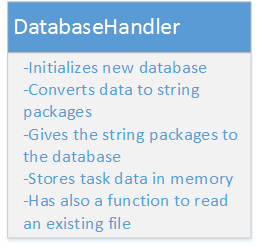
\includegraphics[width=0.3\textwidth]{images/databasehandler.png}
	\begin{itemize}
		\item Provides methods for data parsing
		\item Passes data through
		
	\end{itemize}
	\end{frame}
	
	\begin{frame}{DatabaseServer}
	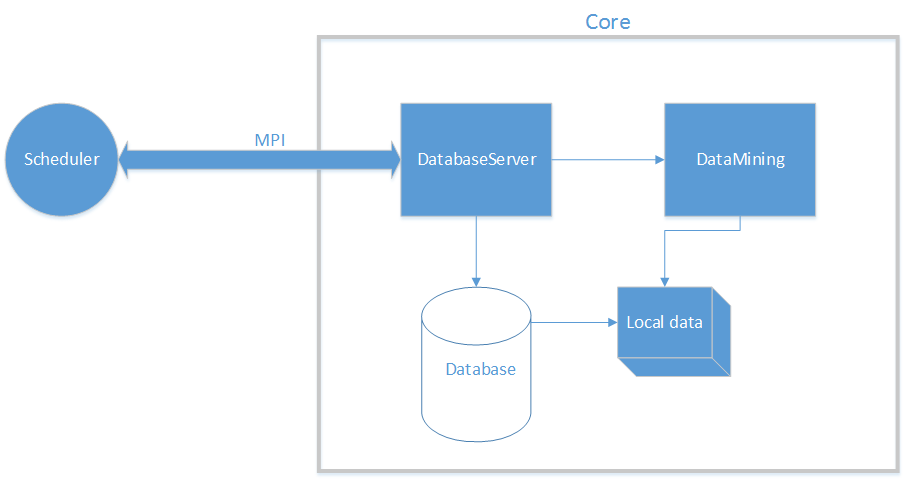
\includegraphics[width=1.0\textwidth]{images/Zeichnung6.png}
	\end{frame}
	
	\begin{frame}{Database - DataMining}
	\centering
	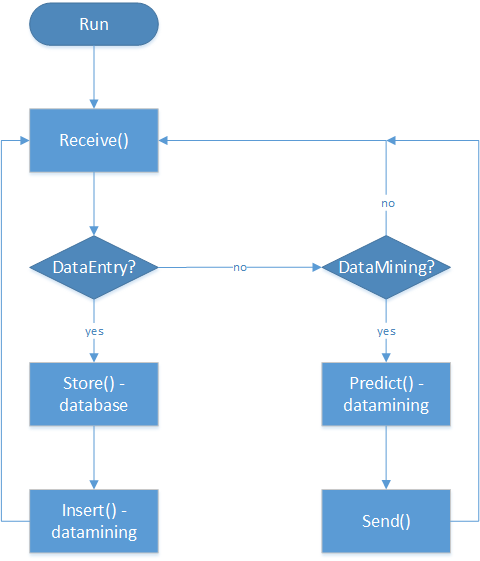
\includegraphics[width=0.55\textwidth]{images/datamining_flow.png}
	\end{frame}
